\documentclass[11pt,a4paper]{ctexart}

\usepackage[margin=2.4cm]{geometry}
\usepackage{amsmath,amssymb}
\usepackage{graphicx}
\usepackage{booktabs}
\usepackage{float}
\usepackage{xcolor}
\usepackage{caption}
\usepackage{tikz}
\usetikzlibrary{arrows.meta}
\usepackage{listings}
\usepackage[hidelinks]{hyperref}

\setCJKmainfont{Noto Serif CJK SC}
\setCJKsansfont{Noto Sans CJK SC}
\setCJKmonofont{Noto Sans Mono CJK SC}

\captionsetup{font=small,labelfont=bf}
\lstset{basicstyle=\ttfamily\small,frame=single,breaklines=true,
        columns=fullflexible,keepspaces=true,showstringspaces=false}

\title{\textbf{Computer Vision (2026 Fall) --- Homework 1}}
\author{姓名：石禾言 \qquad 学号：2500013221}
\date{2026 年 9 月}

\begin{document}
\maketitle

\section{简答题}

\subsection{齐次坐标}

\paragraph{1) 表示同一个笛卡尔点的充要条件与笛卡尔坐标}

设 $\mathbf p=(p_1,\dots,p_N,s)$，$\mathbf q=(q_1,\dots,q_N,t)$，其中 $s,t\neq 0$。
对 $\mathbf p$ 作归一化，得 $\bar{\mathbf p}=(p_1/s,\dots,p_N/s,1)$；
对 $\mathbf q$ 同理得 $\bar{\mathbf q}=(q_1/t,\dots,q_N/t,1)$。

$\mathbf p$ 与 $\mathbf q$ 表示同一个笛卡尔点，当且仅当它们的归一化表示完全相同，即
\begin{equation}
\bar{\mathbf p}=\bar{\mathbf q}
\iff \frac{p_i}{s}=\frac{q_i}{t}\ \ (i=1,\dots,N)
\iff t\,p_i=s\,q_i\ \ (i=1,\dots,N)
\iff \exists\,\lambda\neq 0:\ \mathbf p=\lambda\,\mathbf q,
\end{equation}
其中 $\lambda=s/t$。也就是说，\textbf{充要条件是两个齐次坐标向量成比例}（$s,t\neq 0$）。
该点对应的笛卡尔坐标为 $\bigl(p_1/s,\ p_2/s,\ \dots,\ p_N/s\bigr)$。

这说明齐次坐标表示\textbf{不唯一}：同一个点对应无穷多条过原点的射线上的向量，相差一个非零比例因子。

\paragraph{2) 齐次坐标的两个优点}

\textbf{优点一：把平移与线性变换统一成同一个矩阵乘法。}
在笛卡尔坐标下，仿射变换必须写成 $N$ 维空间中的“线性变换 $+$ 平移”
$\mathbf x\mapsto A\mathbf x+\mathbf b$，它不是 $\mathbb R^N$ 上的线性映射，无法用一个 $N\times N$ 矩阵表示，
复合、求逆都要单独处理平移分量。改用齐次坐标后，同一个变换写成
\begin{equation}
\begin{bmatrix}\mathbf x'\\ 1\end{bmatrix}
=\begin{bmatrix}A&\mathbf b\\ \mathbf 0^\top &1\end{bmatrix}
\begin{bmatrix}\mathbf x\\ 1\end{bmatrix},
\end{equation}
即一个 $(N{+}1)\times(N{+}1)$ 矩阵的乘法。于是所有仿射变换（含平移、旋转、缩放、错切）都成为同一个线性空间上的线性算子，
变换的复合就是矩阵相乘，求逆就是矩阵求逆。

\textbf{优点二：可以统一表示无穷远点（方向）。}
当 $s=0$ 时，齐次向量 $(p_1,\dots,p_N,0)$ 不对应任何有限笛卡尔点，它恰好表示该方向上的\textbf{无穷远点}。
在齐次坐标框架下：
(i) 平行直线也有交点——它们交于无穷远点，因此“任意两条直线必相交”这一射影几何命题无需对平行情形作例外讨论；
(ii) 相机的投影可以写成齐次线性映射，图像的\textbf{消失点/消失线}可以自然表示出来；
(iii) 投影变换可以把无穷远线映射为一条有限直线，实现自由转换。

\subsection{卷帘快门}

设行曝光时间为 $\Delta t_{\text{row}}=T/H$，第 $y$ 行的曝光时刻为 $t(y)=y\,\Delta t_{\text{row}}$（$y$ 自上而下增大），
因此\textbf{图像下方的行曝光更晚}。

\paragraph{1) 列车运动方向的判断}

在卷帘快门图像（图 1 下）中，车门竖直边的下端比上端向\textbf{左}偏移了 $X=200$ 像素。
下端所在的行曝光得更晚，即在下端被曝光的时刻，列车（以及车门边）已经相对上端被曝光的时刻向图像左侧移动了 $200$ 像素。
因此\textbf{列车向左运动}。

\begin{figure}[H]
\centering
\begin{tikzpicture}[x=1.15cm,y=1.15cm,>=Stealth]
  % sheared door edge
  \draw[very thick,orange] (2.4,0) -- (0,-2.0);
  \draw[very thick,orange] (0,0) -- (2.4,0);      % X leg
  \draw[very thick,orange] (0,0) -- (0,-2.0);     % Y leg
  \draw[dashed,gray] (2.4,0) -- (2.4,-2.0);
  \draw[dashed,gray] (0,-2.0) -- (2.4,-2.0);
  % scan direction
  \draw[->,thick,blue] (-1.1,0.25) -- (-1.1,-2.25);
  \node[blue,rotate=90,font=\small] at (-1.55,-1.0) {行曝光方向};
  \foreach \y in {0,-0.4,...,-2.0} \draw[blue] (-1.25,\y) -- (-0.95,\y);
  % labels
  \node[above,font=\small] at (1.2,0.05) {$X=200$ px};
  \node[font=\small,anchor=west,fill=white,inner sep=1.5pt] at (0.12,-1.0) {$Y=300$ px};
  \node[font=\small,align=left,anchor=west] at (2.6,-1.0)
      {卷帘快门下的\\车门竖直边\\(上端靠右、下端靠左)};
\end{tikzpicture}
\caption{卷帘快门造成的竖直边倾斜（对应题目图 1 下半幅）。竖直边的上端曝光更早、下端更晚，
两者水平相差 $X=200$ px、竖直相差 $Y=300$ px；由图中的倾斜方向（上右下左）可知列车向左运动。}
\end{figure}

\paragraph{2) 列车速度的计算}

行曝光时间
\begin{equation}
\Delta t_{\text{row}}=\frac{T}{H}=\frac{30\ \text{ms}}{1000}=0.03\ \text{ms/row}.
\end{equation}
车门边两端所对应的曝光时间差（即曝光完这 $Y=300$ 行所需的时间）
\begin{equation}
\Delta t=Y\cdot\Delta t_{\text{row}}=300\times 0.03\ \text{ms}=9\ \text{ms}=9\times10^{-3}\ \text{s}.
\end{equation}
在这段时间里，车门边在像面上水平移动了 $X$ 像素。由针孔模型，像面上 $x$ 方向的位移 $\Delta x'$ 与深度 $Z$ 处的真实位移 $\Delta X_{\text{real}}$ 满足
$\Delta X_{\text{real}}=\Delta x'\cdot Z/f$，于是
\begin{equation}
\Delta X_{\text{real}}=X\cdot\frac{Z}{f_x}=200\times\frac{15\ \text{m}}{6000}=0.5\ \text{m}.
\end{equation}
列车速度
\begin{equation}
v=\frac{\Delta X_{\text{real}}}{\Delta t}=\frac{0.5\ \text{m}}{9\times10^{-3}\ \text{s}}
=55.6\ \text{m/s}\approx 2.0\times10^{2}\ \text{km/h},
\end{equation}
方向为\textbf{水平向左}（与第 1) 问一致）。合并起来即
\begin{equation}
v=\frac{X\,Z}{f_x\,Y\,\Delta t_{\text{row}}}=\frac{X\,Z\,H}{f_x\,Y\,T}
=\frac{200\times15\times1000}{6000\times300\times30\times10^{-3}}=55.6\ \text{m/s}.
\end{equation}

\section{相机高度}

\subsection{求消失线}

\textbf{方法：} 地面上任意一组平行直线，其像相交于该方向的消失点；地面上两个不同方向的消失点连线即为地面平面的消失线。
由于题目假定相机近似水平且无滚转（镜头畸变忽略），因此\textbf{消失线是一条水平线}，只需确定它的行坐标 $y_h$。

本文取以下两组平行线：
\begin{itemize}
  \item \textbf{组 A（横向，近似平行于像平面）：}广场铺装与车行道之间的长路缘线
  \item \textbf{组 B（沿街道纵深方向）：}左侧花岗岩路缘石带的两条长边——顶边（草地与路缘石的分界）与底边（路缘石与铺装的分界）。
\end{itemize}

由组 A 知消失线水平；组 B 给出消失点应落在该水平线上。设定花坛高 $0.76$ m（图中标注），行人身高约 $1.70$ m。由下节的公式，对任意高度已知的物体都有
$H=h\,(y_{\text{ground}}-y_h)/(y_{\text{ground}}-y_{\text{top}})$，
要求花坛与行人给出同一个相机高度 $H$，由此解出 $y_h\approx1840$，该值同时与组 B 的约束相容。
最终报告消失线为
\begin{equation}
\boxed{\ \text{消失线：水平线，}y_h\approx1840\ \text{像素}\ }
\end{equation}
（像素坐标以图像左上角为原点，$x$ 向右、$y$ 向下；原图尺寸 $4096\times3072$）。
图 \ref{fig:ov} 给出了两组平行线与消失线在图像中的位置。

\begin{figure}[H]
\centering
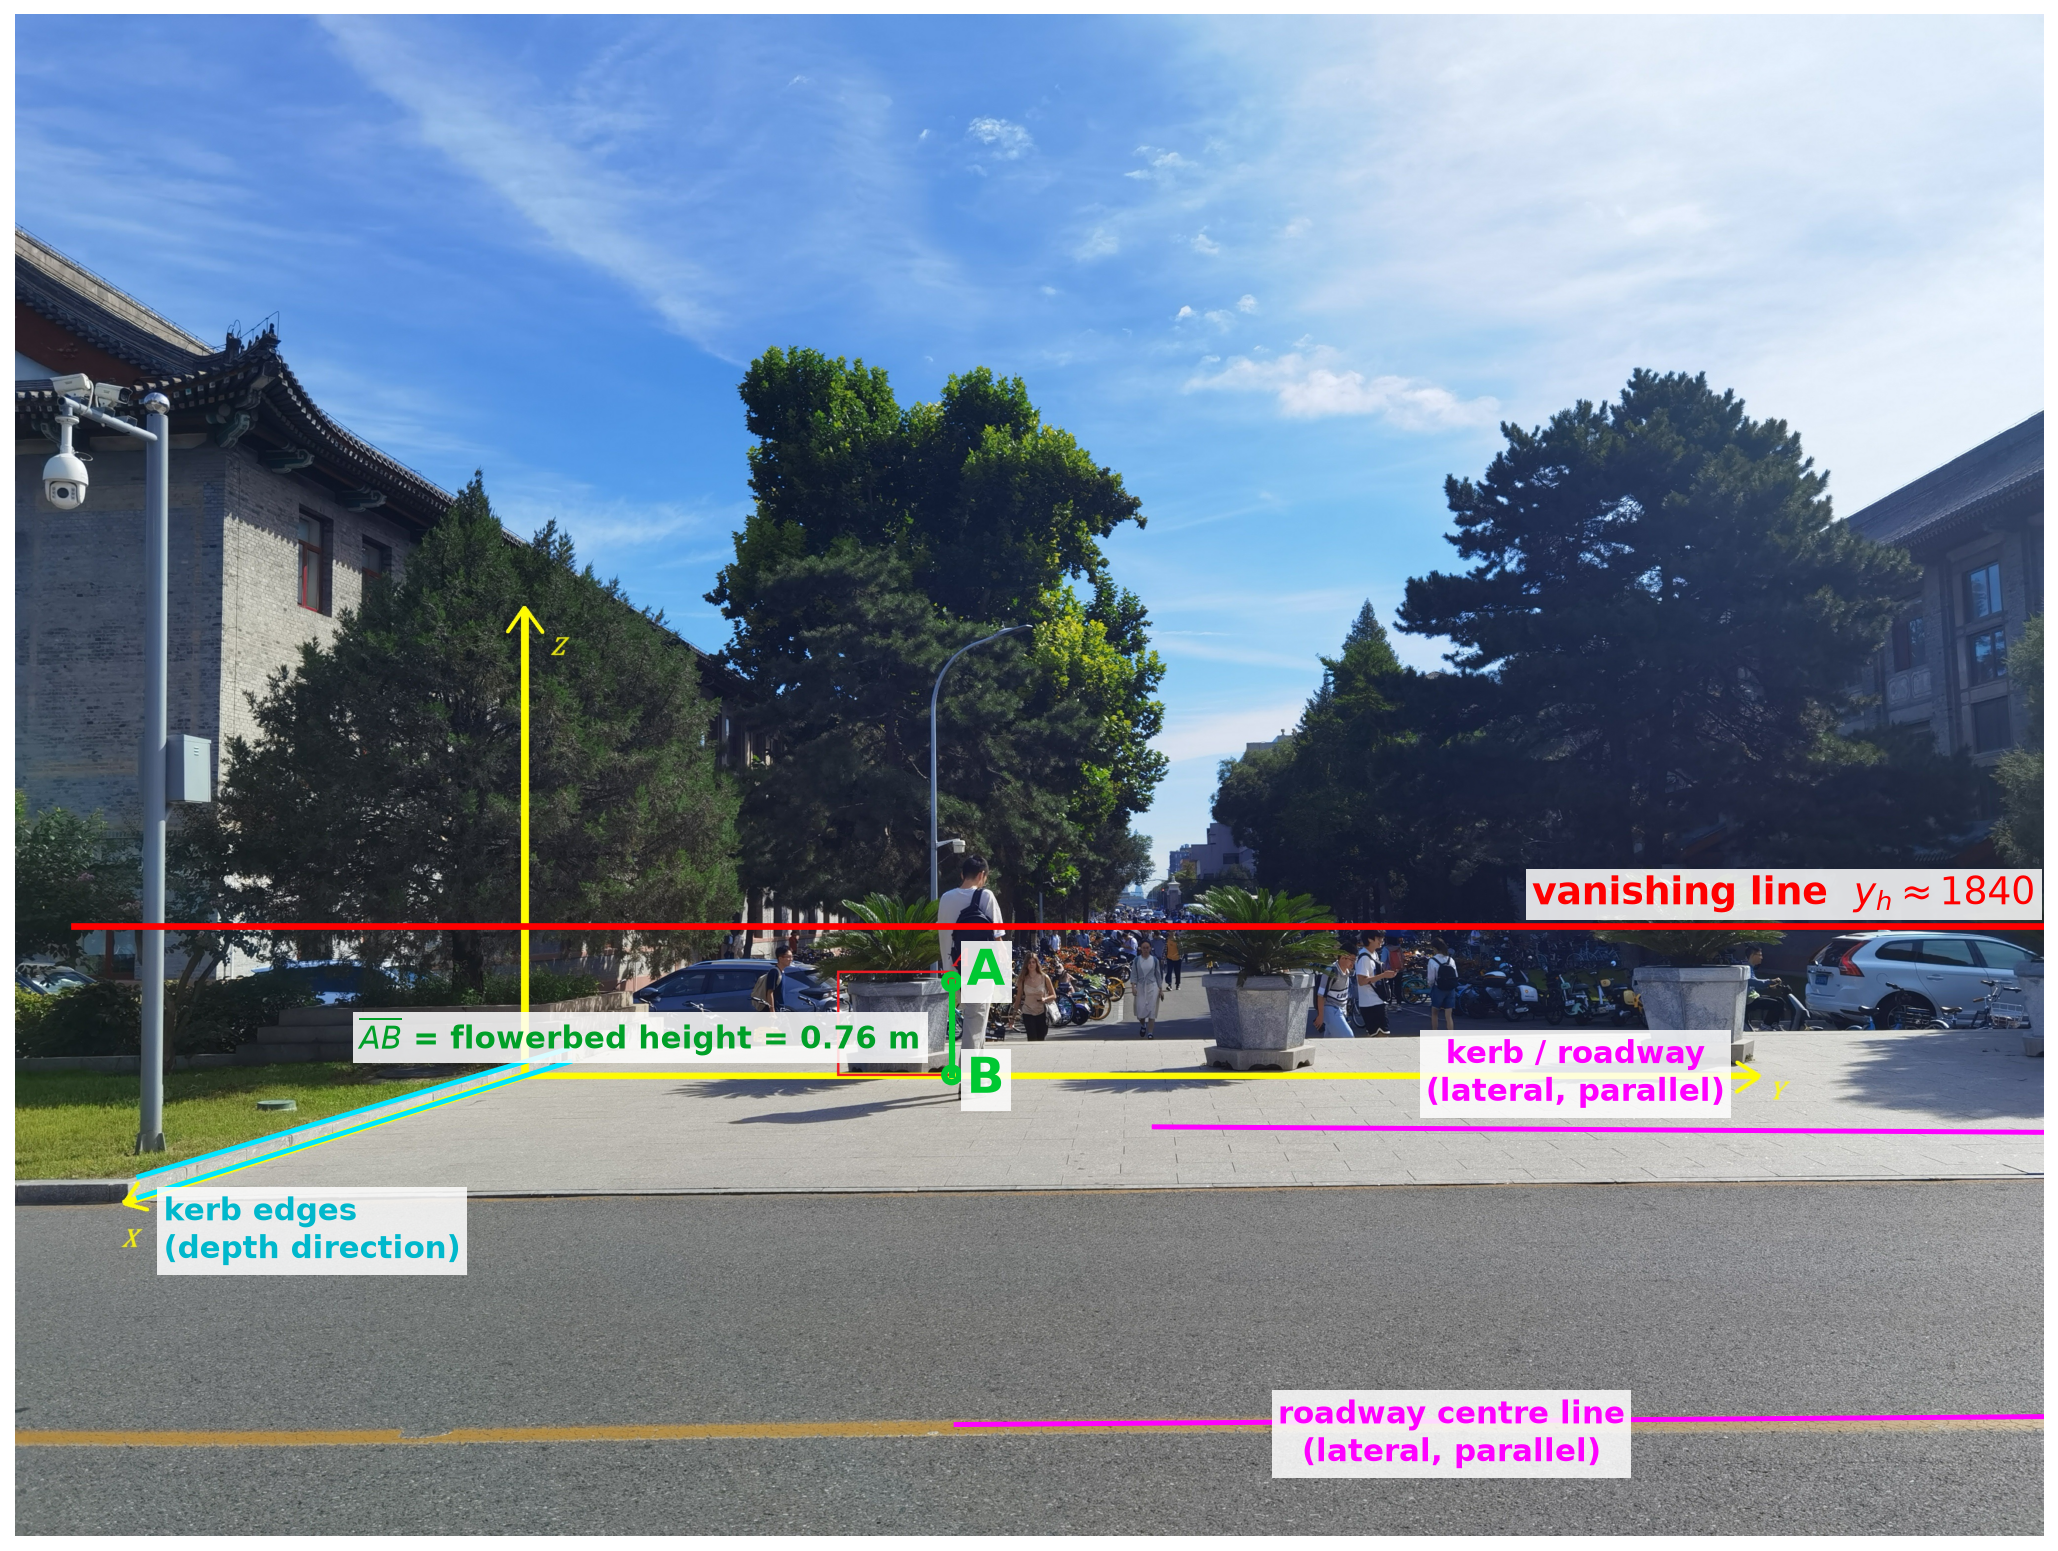
\includegraphics[width=\textwidth]{figs/q2_overview.png}
\caption{消失线的确定。红色水平线为地面平面的消失线（$y_h\approx1840$）；青色为纵深方向的路缘石带两条长边（组 B）；
品红色为两条互相平行的横向长直线（组 A），它们近似水平、消失点在无穷远。绿色线段为花坛上 $A$、$B$ 两点。}
\label{fig:ov}
\end{figure}

\subsection{由参考高度估计相机高度}

\textbf{像素测量。} 在 \texttt{campus.png}（$4096\times3072$）上量得：
\begin{itemize}
  \item $A$：花坛顶沿上的点，$A=(x_A,y_A)=(1891,\ 1953)$；
  \item $B$：$A$ 正下方地面上的点，$B=(x_B,y_B)=(1891,\ 2141)$。
\end{itemize}
由于相机水平无滚转，世界竖直线的像保持竖直，故 $A$、$B$ 在同一像列上：$x_A=x_B=1891$。
它们到消失线的竖直距离为
\begin{equation}
h_1=v_A=y_A-y_h=1953-1840=113\ \text{px},\qquad
h_2=y_B-y_A=2141-1953=188\ \text{px},
\end{equation}
$A$、$B$ 之间的真实距离即花坛高度 $h=0.76$ m。

\textbf{推导。} 设相机光心距地面高 $H$，焦距（像素）$f$，忽略镜头畸变。地面点 $B$ 深度为 $Z$、高度为 $0$，
它在像面上位于消失线下方
\begin{equation}
v_B=\frac{fH}{Z};
\end{equation}
花坛顶沿上的点 $A$ 与 $B$ 在同一竖直线上（深度同为 $Z$）、高出地面 $h$，
\begin{equation}
v_A=\frac{f(H-h)}{Z}.
\end{equation}
两式相除，$f$ 与 $Z$ 同时消去：
\begin{equation}
\frac{v_A}{v_B}=\frac{H-h}{H}=1-\frac{h}{H}
\quad\Longrightarrow\quad
\boxed{\,H=h\cdot\frac{v_B}{v_B-v_A}=h\cdot\frac{h_1+h_2}{h_2}\,}
\end{equation}
这与前置知识中的构造一致：$h_1$ 是消失线到 $A$ 的距离，$h_2$ 是 $A$ 到 $B$ 的距离。
代入数值（$v_B=h_1+h_2=113+188=301$，$v_B-v_A=h_2=188$）：
\begin{equation}
H=0.76\times\frac{301}{188}=0.76\times1.601=1.22\ \text{m}
\;\approx\;1.2\ \text{m}.
\end{equation}

\begin{figure}[H]
\centering
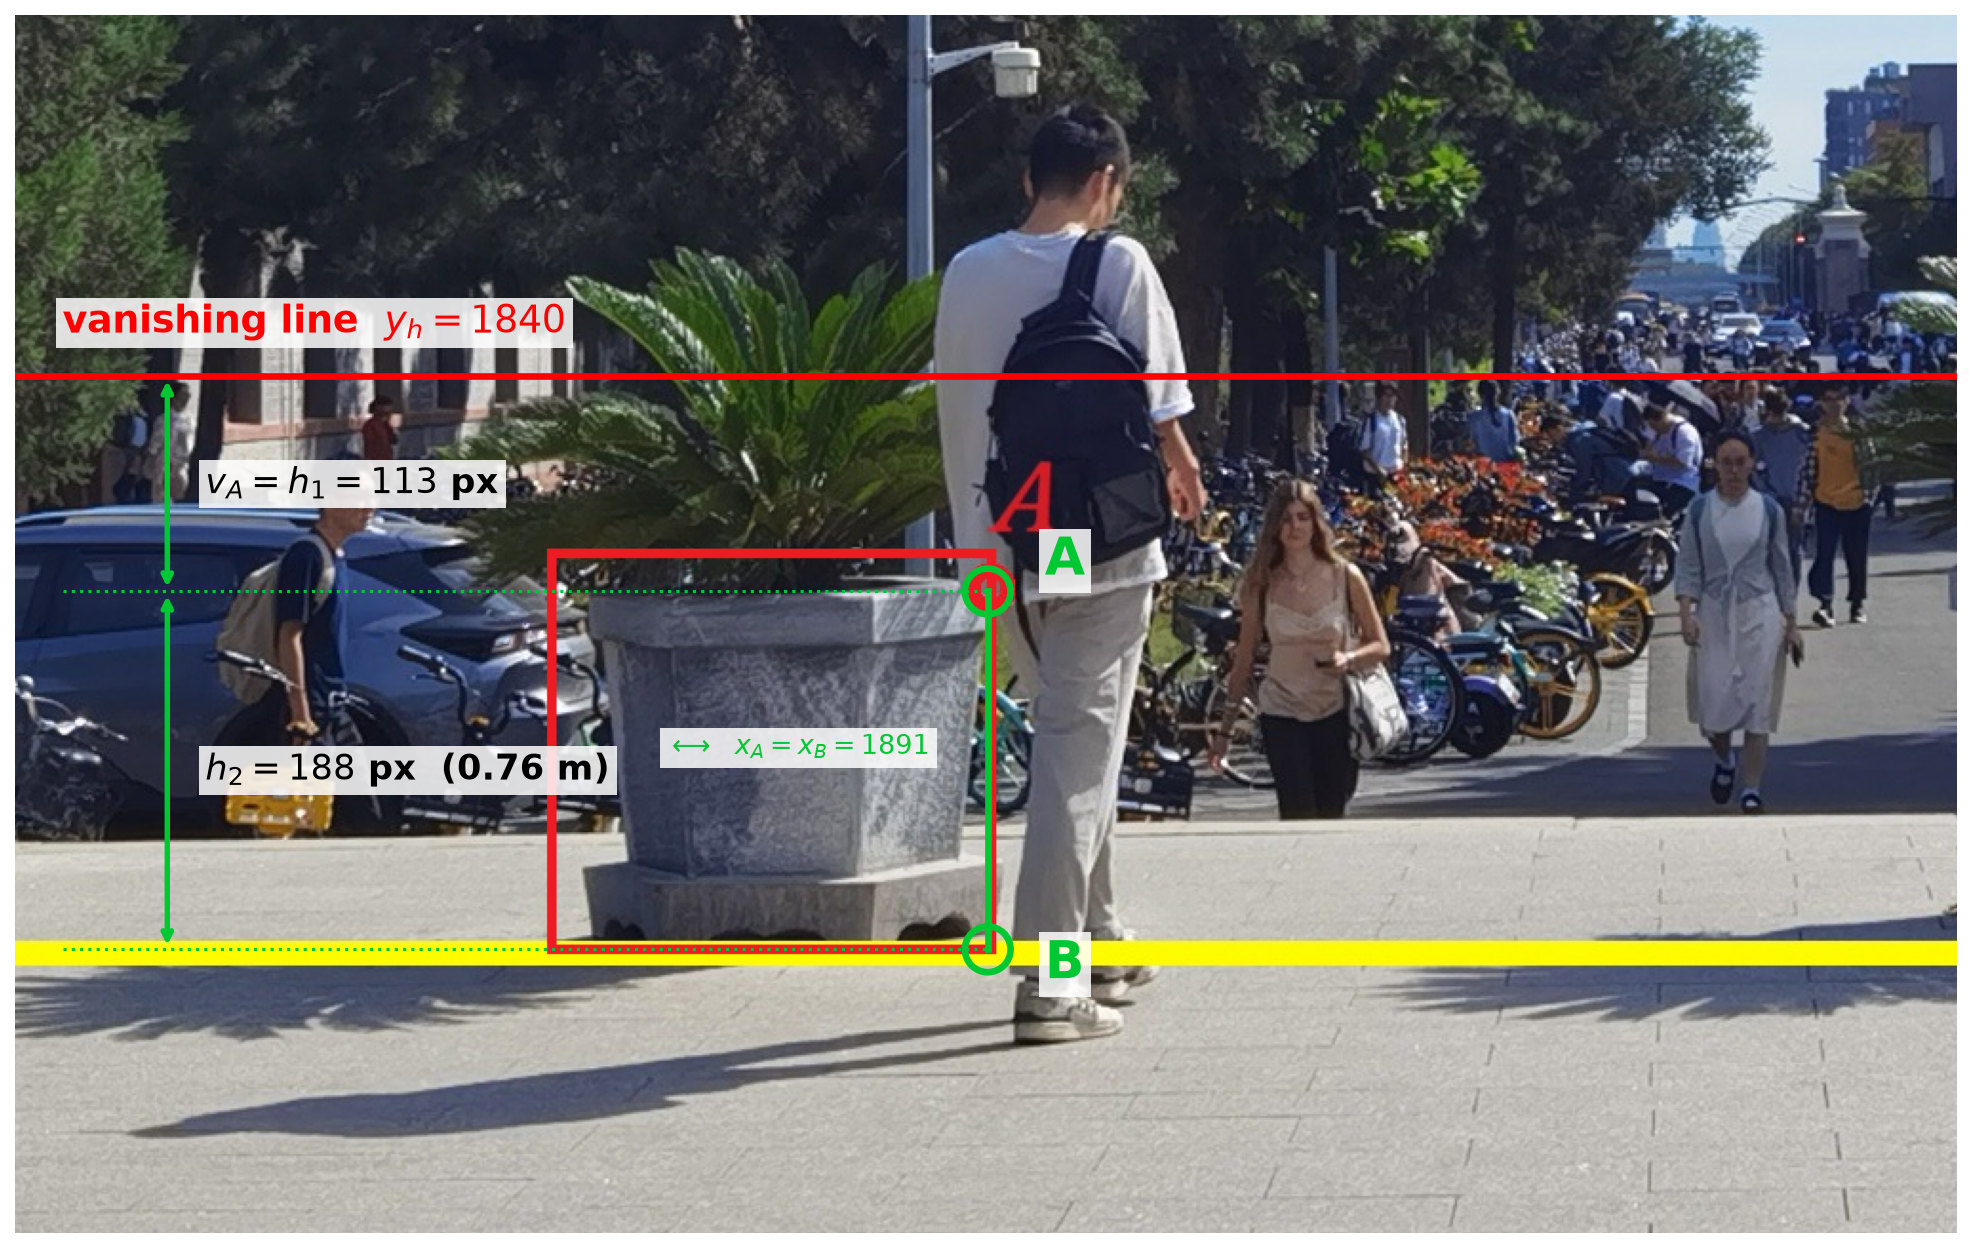
\includegraphics[width=\textwidth]{figs/q2_zoom.png}
\caption{$A$、$B$ 与消失线（局部放大）。$A=(1891,1953)$ 在花坛顶沿上，$B=(1891,2141)$ 是 $A$ 正下方的地面点，
二者对应的真实距离为花坛高度 $0.76$ m；$v_A=h_1=113$ px，$h_2=188$ px，$H=0.76\,(h_1+h_2)/h_2\approx1.2$ m。}
\label{fig:zoom}
\end{figure}

\section{图像滤波与降采样}

\subsection{实现说明}

所有函数均由本人用 NumPy 实现：

\begin{itemize}
  \item \texttt{cross\_correlation\_2d}$(f,h)$：不翻转核，按
        $g(i,j)=\sum_{k,l} f(i+k,\,j+l)\,h(k,l)$ 逐位移加权求和（用 \texttt{np.pad} 做边界填充）；
  \item \texttt{convolve\_2d}$(f,h)$：把核的两个轴都翻转后调用相关函数，即
        $g(i,j)=\sum_{k,l} f(i-k,\,j-l)\,h(k,l)$；
  \item \texttt{gaussian\_blur\_kernel\_2d}$(k,\sigma)$：$h(x,y)=\frac{1}{2\pi\sigma^{2}}
        e^{-(x^{2}+y^{2})/(2\sigma^{2})}$，$(x,y)$ 取 $[-\frac{k-1}{2},\frac{k-1}{2}]$ 的整数网格，并归一化使和为 $1$；
  \item \texttt{low\_pass}：用上面的核与 \texttt{convolve\_2d} 卷积（另提供可分离版本 \texttt{low\_pass\_separable} 作一致性检查，
        两者最大绝对差 $2.0\times10^{-13}$，仅为浮点舍入误差）；
  \item \texttt{image\_subsampling}$(f,s)$：按因子 $s$ 丢弃行与列，即 $f[::s,::s]$，尺寸变为 $(M/s)\times(N/s)$；
  \item \texttt{gaussian\_pyramid}：每一级先低通、再以因子 $2$ 降采样，得到原图及约 $1/2,1/4,1/8$ 分辨率的四级。
\end{itemize}

\textbf{依赖与运行方式：} 需要 \texttt{numpy}（数组运算）、\texttt{Pillow}（读写图像）、\texttt{matplotlib}（输出对比图）。
在脚本所在目录下运行
\begin{lstlisting}
python3 gaussian_pyramid.py                      # 默认输入 ./zebra.jpg，输出到 ./out
python3 gaussian_pyramid.py --image zebra.jpg --outdir out --kernel 5 --sigma 1.0
\end{lstlisting}
输入输出均使用相对路径。脚本会在 \texttt{./out/} 下分别保存 \texttt{gaussian\_pyramid/} 与 \texttt{direct\_pyramid/} 两个金字塔的
$1/2,1/4,1/8$ 各级图像，并生成对比图 \texttt{./out/comparison.png}。

\subsection{滤波金字塔与直接降采样的对比}

对同一张纹理图像 \texttt{zebra.jpg}（$534\times400$，RGB 三通道，未转灰度）分别构造
(a) 高斯金字塔：每级先做 $5\times5,\ \sigma=1.0$ 的高斯低通再隔行隔列抽样；
(b) 直接金字塔：每级直接隔行隔列抽样，不做任何平滑。

\begin{table}[H]
\centering
\caption{两个金字塔对应级别之间的差异（逐像素绝对差），以及各级的高频能量
（HF $=$ Laplacian 绝对值的均值，数值越大高频成分越多）。}
\small
\setlength{\tabcolsep}{5pt}
\begin{tabular}{lcccccc}
\toprule
级别 & 尺寸 & MAE & 最大绝对差 & $>$16 的比例 & HF（高斯） & HF（直接）\\
\midrule
$1/2$     & $267\times200$ & 6.53  & 83.1  & 9.4\%  & 18.58 & 41.78\\
$1/4$     & $134\times100$ & 12.42 & 126.4 & 23.1\% & 21.60 & 60.96\\
$1/8$     & $67\times50$   & 18.87 & 116.6 & 35.2\% & 21.64 & 85.47\\
\bottomrule
\end{tabular}
\end{table}

\textbf{结论：两者明显不同，且差异随层数增大。} 目视对比（图 \ref{fig:cmp}）可以看到：
高斯金字塔的各级图像平滑、结构完整；而直接降采样得到的图像出现了明显的锯齿、摩尔纹，分辨率越低越严重
（$1/8$ 级最明显）。定量地看，直接降采样结果的高频能量在每一级都远高于高斯金字塔（$1/8$ 级为 $85.5$ 对 $21.6$），
且与高斯的逐像素差异（MAE $6.53\to18.87$，$>$16 的像素从 $9.4\%$ 升到 $35.2\%$）随层数单调增大。

\textbf{原因（混叠）。} 
\texttt{zebra.jpg} 的条纹本身含有大量接近像素级的高频成分。隔行隔列抽样不会使高频分量消失，而是\textbf{折叠}到低频，
在图像中表现为原来不存在的粗条纹、摩尔纹和锯齿。
高斯低通滤波使得每一级都保持了较低的、稳定的高频能量。直接降采样没有这一步，混叠误差会在逐级降采样中不断累积，
所以层数越高差异越大。

\begin{figure}[H]
\centering
\includegraphics[width=\textwidth]{figs/q3_comparison.png}
\caption{上排为高斯金字塔（先低通再降采样），下排为直接降采样金字塔。
直接降采样各级（尤其 $1/4$、$1/8$）出现明显的锯齿与摩尔纹，即混叠伪影。}
\label{fig:cmp}
\end{figure}

\section{AI 使用声明}

\begin{itemize}
  \item 第 1 题（齐次坐标、卷帘快门）的解答由本人完成，AI 仅协助将其手写稿整理为 \LaTeX{} 排版。
  \item 第 2 题（相机高度）在 \texttt{campus.png} 上提取路缘石边缘、
        标定像素坐标（$A$、$B$、消失线）等工作借助 AI 辅助完成，用于校验测量结果。
  \item 第 3 题中第 3.1--3.4 节要求的六个函数由本人实现，
        即 \texttt{cross\_correlation\_2d}、\texttt{convolve\_2d} 等六个滤波与金字塔函数；
        \texttt{main()} 中的API接口和调用代码由 AI 协助完成。
  \item 本报告的 \LaTeX{} 排版由 AI 协助完成。所有由 AI 协助产生的内容均已由本人核对、运行与修改。
\end{itemize}

\end{document}
